\chapter{CORDIC}

En este capítulo veremos el funcionamiento de \glossary{cordic} básico, algunas posibles mejoras y el caso específico de tratamiento de datos en punto flotante.

\section{Descripción de \gls{cordic}}

En esta sección se describirá el funcionamiento principal del algoritmo \gls{cordic} según descrito por \cite{volder_cordic_1959}.

La rotación de un vector de dos dimensiones $\boldsymbol{p_{0}} = [x_{0},y_{0}]$ con un ángulo $\theta$ para obtener un vector $\boldsymbol{p_{n}} = [x_{n},y_{n}]$ se puede realizar con un producto matriz $\boldsymbol{p_{n}}$ = $\boldsymbol{R_{p_{0}}}$, donde $\textbf{R}$ es la matriz de rotación.

\[ \textbf{R} = \begin{bmatrix}
\cos{\theta} & -\sin{\theta} 	\\[0.3em]
\sin{\theta}  & \cos{\theta} 			\\[0.3em]
\end{bmatrix} \]

Si sacamos el coseno de la matriz de rotación, se puede obtener un valor K, el cual se convierte en una constante.

\[ \textbf{R} = [(1 + \tan^2{\theta})^{\sfrac{-1}{2}}] \begin{bmatrix}
1 & -\tan{\theta} 	\\[0.3em]
\tan{\theta}  & 1 			\\[0.3em]
\end{bmatrix} \]

Nombraremos como $K = [(1 + \tan^2{\theta})^{\sfrac{-1}{2}}]$ el factor escala. Eliminando $K$ obtenemos una matriz de pseudo-rotación $\boldsymbol{R_{c}}$ tal que

\[ \boldsymbol{R_{c}} = \begin{bmatrix}
1 & -\tan{\theta} 	\\[0.3em]
\tan{\theta}  & 1 			\\[0.3em]
\end{bmatrix} \]

La operación pseudo-rotación rota el vector $p_{0}$ por un ángulo $\theta$ y cambia su magnitud por un factor $K = \cos{\theta}$ para producir una pseudo-rotación $p'_n = R_c p_0$.

Para obtener la simplicidad dentro del hardware necesitamos:

\begin{itemize}
	\item Descomponer las rotaciones en una secuencia de rotaciones elementales con ángulos predefinidos que se pueda implementar con un coste hardware mínimo.
	\item Eliminar el factor escala $K$, ya sea finalizando la operación con una simple multiplicación o ignorándolo directamente.
\end{itemize}

En primer lugar, \gls{cordic} realiza una rotación iterativa con una lista de ángulos predefinidos $\alpha_{i} = \arctan({2^{-i}})$ de manera que $\tan({\alpha_{i}}) = 2^{-i}$ se puede implementar en hardware como un desplazamiento de $i$ posiciones.

Ya que estamos limitando la operación $\tan{\theta}$ a una lista de rangos predefinidos anteriormente podemos asumir que

\[
	K_{i} = \frac{1}{sqrt{(1+2^{-2_{i}})}}
\]

El factor escala $K_{i}$ altera la magnitud del vector a rotar independientemente del valor del ángulo. 

Ya que el factor escala no depende del ángulo de las micro-rotaciones, no necesitamos incluir el factor dentro de las operaciones, lo que nos da $\boldmath{p_{n} = R_{c}p_{0}}$.

El factor final $K \approx 1.6467605$, por lo cual simplemente se puede escalar el valor final por $K$.

Los valores finales que nos interesan son los siguientes:

\[
\begin{matrix}
	x_{i+1} = x_{i} - \delta_{i} \times 2^{-i} \times y_{i} \\
	y_{i+1} = y_{i} - \delta_{i} \times 2^{-i} \times x_{i} \\
	\omega_{i+1} =  \omega_{i} - \delta_{i} \times \alpha_{i}
\end{matrix}
\]

\begin{figure}[ht]
	\centering
	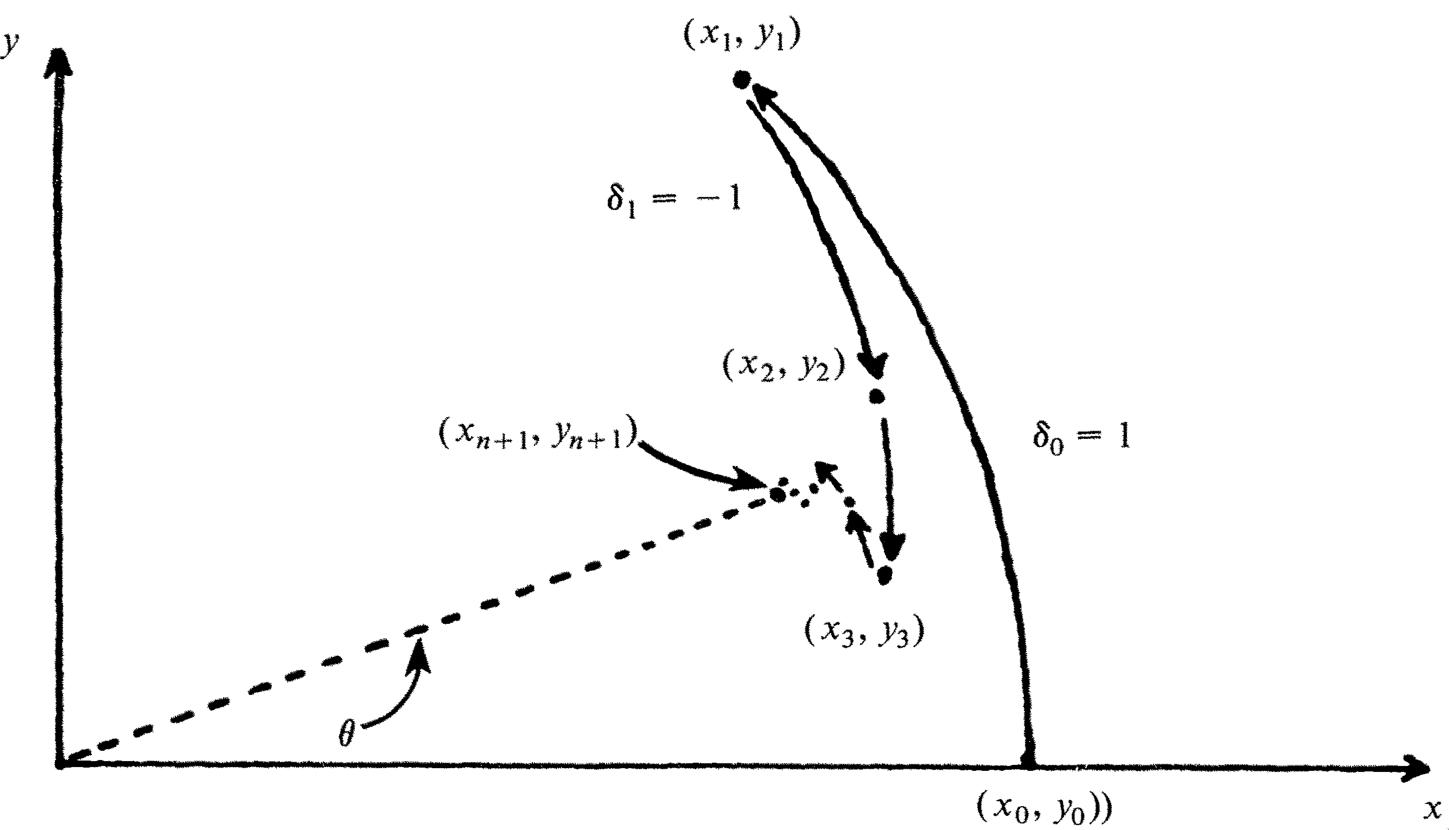
\includegraphics[width=\textwidth]{archivos/CORDIC/RotationMode.png}
	\caption{Rotation Mode. Figura de \cite{schelin_calculator_1983}}
	\label{graf:RM}
\end{figure}

\begin{figure}[ht]
	\centering
	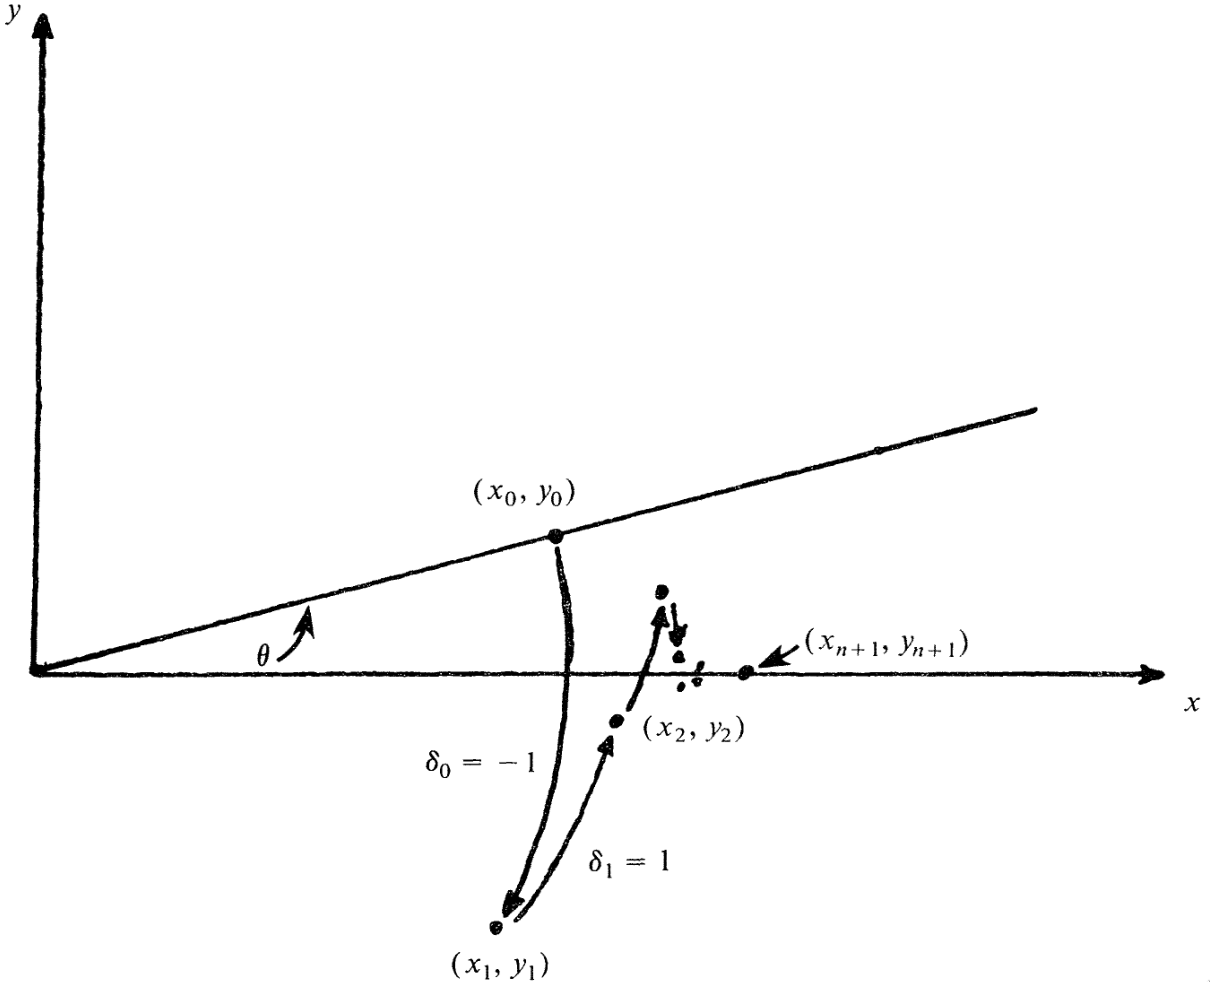
\includegraphics[width=\textwidth]{archivos/CORDIC/VectoringMode.png}
	\caption{Vectoring Mode. Figura de \cite{schelin_calculator_1983}}
	\label{graf:VM}
\end{figure}

\gls{cordic} puede operar de dos formas: \textit{Rotation Mode} (RM) (Figura \ref{graf:RM}) y \textit{Vectoring Mode} (VM) (Figura \ref{graf:VM}). La principal diferencia es en como se eligen las micro-rotaciones. En RM, la dirección de cada micro-rotación depende del signo de $\omega_{i}$. Si $\omega_{i}$ es positivo $\delta_{i} = 1$, si no $\delta_{i} = -1$. En VM, el vector rota hacia el eje de $x$, por lo que la componente $y$ tiende a 0.

Posteriormente, J.S. Walther propuso un \gls{cordic} generalizado unificado para realizar multitud de operaciones matemáticas. La tabla \ref{table:2009-CORDIC-Configurations} muestra las diferentes configuraciones que puede tener \gls{cordic} para obtener un tipo de operación u otro. Esto se encuentra fuera del alcance de esta memoria, pero se ha querido mostrar la amplitud del método para casos de uso diferentes.

\begin{table}[]
	\centering
	\resizebox{\textwidth}{!}{%
		\begin{tabular}{|l|l|l|l|l|}
			\hline
			\textbf{Operación}   & \textbf{Configuración} & \textbf{Inicialización} & \textbf{Salida} & \textbf{Anotaciones} \\ \hline
			$\cos\theta, \cos\theta, \tan\theta$ & CC-RM         & $x_0 = 1 $ $ y_0 = 0$ y $\omega_0 = \theta$           & $x_=\cos\theta$ $ y_n = \sin\theta $  & $\tan\theta = (\sin\theta/\cos\theta) $       \\ \hline
			
			$\cosh\theta, \sinh\theta,\tanh\theta,\exp(\theta)$& HC-RM               & $x_0 = 1$ $ y_0 = 0 $ y $\omega_0 = \theta$               & $x_n = \cos\theta$ $ y_n = \sinh\theta $        & $x_n = \sqrt{a} $ $\omega_n = 1/2\ln(a)$            \\ \hline
			
			$\ln(a),\sqrt{a}$& HC-VM               & $x_0 = a+1 $ $ y_0 = a-1 $ y $\omega_0 = 0$                 & $x_n = \sqrt{a}$ $ \omega_n=1/2\ln{a}$         & $\ln(a)=2\omega_n$            \\ \hline
			
			$\arctan(a)$& CC-VM              & $x_0 = a$ $ y_0 = 1 $ y $\omega_0 = 0$               & $\omega_n = \arctan(a) $        &             \\ \hline
			
			división$(b/a)$& LC-VM              &$x_0 = a$ $ y_0 = b$ y $\omega_0 = 0$                &  $\omega_n = b/a$       &             \\ \hline
			
			Polar a rectangular& CC-RM             &$x_0 = R$ $ y_0 = 0 $ y $\omega_0 = \theta$             & $x_n = R\cos\theta $ $ y_n = R\sin\theta$       &             \\ \hline
			
			Rectangular a polar $\tan^-1(b/a)$ y $\sqrt{a^2+b^2}$& CC-VM               & $ x_0 = a$ $ y_0 = b$ y $\omega_0 = 0$     &$x_n = \sqrt{a^2 + b^2} $ $ \omega_n = \arctan(b/a)$        &             \\ \hline
			
		\end{tabular}%
	}
	\caption{Diferentes configuraciones de \gls{cordic}, segun \cite{meher_50_2009}}
	\label{table:2009-CORDIC-Configurations}
\end{table}

\section{Mejoras a CORDIC}
En el apartado de introducción se explicaron algunas aplicaciones de \gls{cordic}, sin detallar el tipo o las modificaciones realizadas. En este apartado se muestran algunas de estas mejoras importantes que han permitido a \gls{cordic} mantenerse competitivo. Muchas de estas soluciones están descritas en \cite{meher_50_2009}, y expuestas en la tabla \ref{table:2009-CORDIC-Configurations}.

Como ya se comentó anteriormente, el cómputo de \gls{cordic} es originalmente un proceso totalmente secuencial por dos razones principales: las micro-rotaciones depende de los valores la rotación computados anteriormente, lo que sería el valor intermedio y la iteración $(i+1)$ solo puede comenzar después de que se complete la iteración $i$.

Otro de los problemas es que la precisión del valor final es lineal, requiere $n+1$ iteraciones para tener una precisión de $n$ bits. Esto significa que la latencia depende del número de bits que se pasan a \gls{cordic}.

\subsection{4-Radix}
Una solución a la reducción del número de iteraciones es calcular \gls{cordic} con una base mayor, como por ejemplo 4 (\cite{antelo_high_1997}) La fórmula final seria tal que:

\[
\begin{matrix}
x_{i+1} = x_{i} - \delta_{i} \times 4^{-i} \times y_{i} \\
y_{i+1} = y_{i} - \delta_{i} \times 4^{-i} \times x_{i} \\
\omega_{i+1} =  \omega_{i} - \delta_{i} \times \alpha_{i}
\end{matrix}
\]

El valor $K$ tendría una fórmula:

\[
K_{i} = \frac{1}{sqrt{(1+\delta_i^2*4^{-2_{i}})}}
\]

De esta manera, para tener una salida de $n$ bits de precisión solo necesitamos $n/2$ micro-rotaciones a cambio de mas complejidad dentro del hardware. Un punto a comentar es que el factor de escala $K$ ahora depende de $\delta$, el cual puede tener 5 valores diferentes.

También existen soluciones de base mas alto, como 8-Radix.

\subsection{Angle Recording}
Los métodos de \textit{Angle Recording} (AR) quieren reducir el número de iteraciones mediante una combinación lineal de los ángulos de las micro-rotaciones. Este método es ideal para procesamiento de señal, imagen, donde el ángulo de rotación se conoce \textit{a priori}. Algunos métodos consiguen reducir hasta un $50\%$ el número de iteraciones, manteniendo la misma precisión. \cite{hu_angle_1993}

\subsection{Hybrid \glsentryshort{cordic}}
\glsentryshort{cordic} híbrido se basa en la idea de que los valores menos significativos del cálculo de ángulo pueden ser reemplazados por $2^{-j}$ ya que $\tan(2^{-j}) \approx 2^{-j} $ si el valor $j$ es lo suficientemente grande. De esta manera podemos calcular los valores mas pequeños con un simple movimiento de bits y no necesitamos conocer el signo de rotación ya que en todo momento es positivo. \cite{wang_hybrid_1997}

\subsection{Redundant-Number-Based \glsentryshort{cordic}}
Este tipo de \gls{cordic} pretende mejorar el rendimiento de las sumas y restas mediante un uso de numeración redundante para no tener que realizar el cálculo de los posibles restos que puede obtener una operación aritmética. La desventaja de este método es que necesitas mas espacio en hardware para implementar. \cite{ercegovac_redundant_1990}

\subsection{Pipelined \glsentryshort{cordic}}
El uso de \textit{pipelined} \gls{cordic} es bastante extenso ya que cada iteración del método es idéntica y los valores anteriores después de su cálculo ya no nos interesan, por lo que podemos aprovechar esta propiedad para calcular un nuevo valor por cada ciclo de ejecución, dando lugar a un nuevo resultado. Para esto necesitamos tener un registro por cada etapa de \gls{cordic} (vea la figura \ref{graf:2009-CORDIC_pipelined}.).

\begin{figure}[ht]
	\centering
	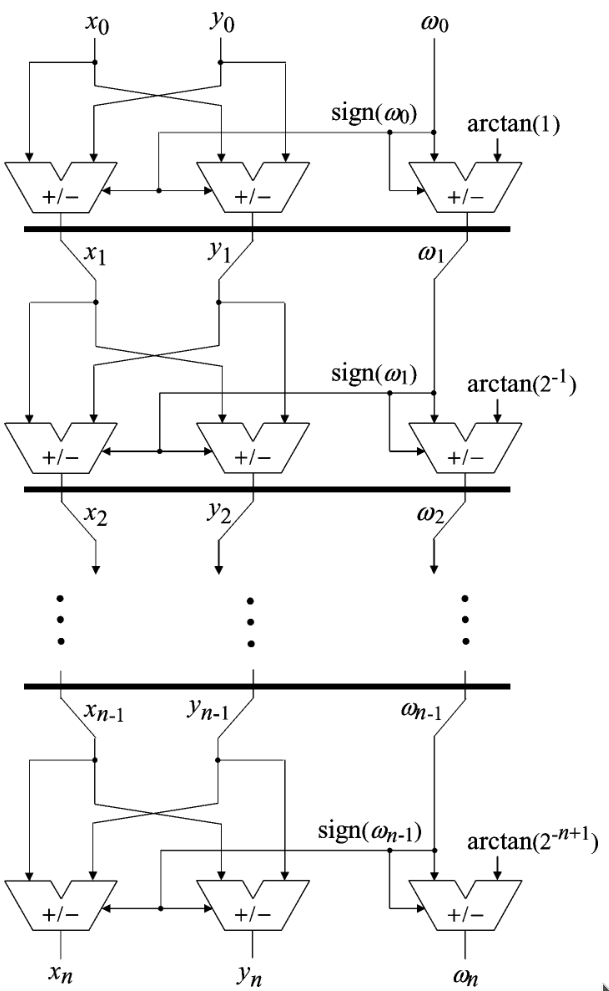
\includegraphics[width=0.50\textwidth]{archivos/CORDIC/2009-CORDIC_pipelined.png}
	\caption{\gls{cordic} convencional con \textit{pipelining}. Extraído de \cite{meher_50_2009}}
	\label{graf:2009-CORDIC_pipelined}
\end{figure}

\section{\glsentryshort{cordic} y punto flotante}

\cite{parker_abstract_2011} Muestra claramente algunos de los problemas que conlleva implementar el estándar del \gls{ieee} 754 en hardware. En concreto estos problemas son relaciones con algunos aspectos de las \gls{fpga}s, pero puede ser aplicable a cualquier problema donde el hardware es limitado. Algunos de estos problemas son:

\begin{itemize}
	\item La representación de la mantisa incluye un 1 implícito. El valor real va desde [1:1.999..] en vez de [0:0.000..]. 
	\item En vez de usar complemento a dos, el estándar incluye un bit de signo.
	\item Cada operación aritmética conlleva una normalización de la mantisa para alinear el punto decimal hacia la izquierda, además de tener que ajustar el exponente de forma acorde.
	\item \gls{vhdl} y Verilog no tienen una implementación de operaciones con punto flotante. Un lenguaje de descripción de hardware más nuevo, como SystemVerilog, sí tiene estas operaciones, pero la complejidad de ellas conlleva a perder mucho espacio, el cual puede estar bastante limitado en las \gls{fpga}s.
\end{itemize}

Dentro de la evolución del uso de punto flotante en el método hay una variedad importante de arquitecturas y algoritmos de \gls{cordic}.

Una de las primeras implementaciones de un tipo de punto flotante, explicado por \cite{leibson_9100_2005} fue sobre el año 1954 con la calculadora de sobremesa HP 9100A. La calculadora tenía 16 registros, numerados de forma hexadecimal y podía guardar valores de punto flotante con 10 dígitos de mantisa y 2 dígitos de exponente en formato \gls{bcd}. La mantisa y el exponente podían guardar valores positivos y negativos.

Según \cite{walther_unified_1971}, la primera implementación de punto flotante tenía grandes limitaciones en el tema de hardware a la hora de convertir los valores entre \gls{bcd} a base 2 y, además, no había un estándar de punto flotante en aquel entonces, por lo que cada diseñador creaba su propio formato.

Un diseño de \gls{cordic} que mas se asemeja a las nuevas propuestas es el de \cite{de_lange_optimal_1988}, donde proponen un procesador de \gls{cordic} de punto flotante y con \textit{pipelining} . Este chip podía realizar hasta $10^7$ rotaciones por segundo gracias al sistema de \textit{pipelining}. La entrada de valores era de 21 bits en punto flotante, 16 bits de mantisa y 5 bits para el exponente en complemento a dos. La salida era también en punto flotante (vea la figura \ref{graf:Arq_FP_CORDIC}). Cabe destacar que el tipo usado en esta arquitectura no es estándar de \gls{ieee} 754.

\begin{figure}[ht]
	\centering
	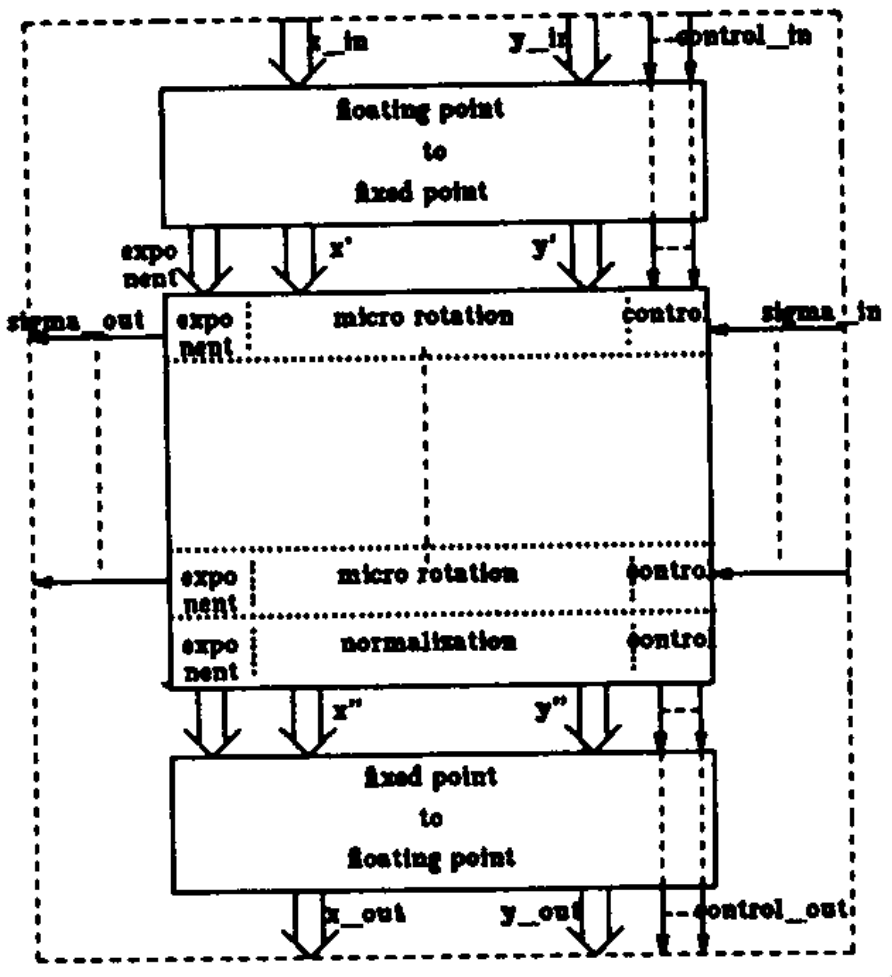
\includegraphics[width=0.5\textwidth]{archivos/CORDIC/1988_FP_CORDIC_Architecture.png}
	\caption{Arquitectura de FP \gls{cordic}. Figura de \cite{de_lange_optimal_1988}}
	\label{graf:Arq_FP_CORDIC}
\end{figure}

Para realizar las micro-rotaciones estipuladas anteriormente, la base del propio algoritmo, el procesador transforma el valor de punto flotante en punto fijo para el trabajo interno y posteriormente devuelve los valores en punto flotante. El valor $K$ es calculado en el momento de la conversión final del valor para devolver.

Como se puede observar, operar con punto fijo para realizar movimiento de bits es mucho mas fácil que tener que hacerlo directamente con punto flotante, por lo que los diseñadores generalmente, en muchos de los ejemplos mostrados posteriormente, realizan una conversión de punto fijo a punto flotante, o algunas veces directamente reciben valores en punto fijo para simplemente convertir una sola vez a punto flotante al final del algoritmo (vea la tabla \ref{table:FP_CORDIC_feature}).

\begin{table}[]
	\centering
	\begin{tabular}{|l|l|l|l|l|}
		\hline
		Precisión & Rango                 & Throughput & Latencia                  & Transistores \\ \hline
		16-bits   & $\pm2^{16}$ & 100ns      & 2.2 $\mu$s                     & 70000        \\
		\hline
		Entradas  & Salidas               & Consumo    & Espacio                   & Procesador   \\ \hline
		72        & 67                    & 1.3W       & 1.2 $cm^2$ & CMOS(2$\mu$) \\ \hline   
	\end{tabular}
	\caption{Características de FP CORDIC. Datos de \cite{de_lange_optimal_1988}}
	\label{table:FP_CORDIC_feature}
\end{table}

\cite{hekstra_floating_1993} presentaron un algoritmo de \gls{cordic} de 32 bit de precisión con el estándar de \gls{ieee} 754. Este algoritmo puede realizar la rotación de un vector punto flotante $(x,y)$ con un ángulo de punto flotante $\alpha$. Este algoritmo fue diseñado con la intención de implementarlo en una unidad funcional para aplicaciones de procesamiento digital (\gls{dsp}).

Para realizar las micro-rotaciones se da ciertos cambios, como el uso del método \textit{Block Floating Point} (BFP) (vea \cite{noauthor_fftifft_2005}), el cual permite un uso de aritmética con punto fijo aunque el valor sea punto flotante. La ventaja de este método es la reducción de hardware y el coste de tiempo que puede traer las mismas funciones aritméticas comparadas a punto flotante pero sin perder el rango numérico que le da la ventaja a este.

\cite{zhou_double_2008} diseñaron un co-procesador \gls{fpga} basado en \gls{cordic} con doble precisión (64 bits estándar \gls{ieee} 754) y \textit{pipelining}. Este diseño se centra explícitamente en las \gls{fpga}s, ya que como se puede ver anteriormente, y según lo descrito en este artículo, la mayoría se centraba dentro del área del \gls{asic}, por lo que no había tantos ejemplos de implementaciones en hardware para \gls{fpga}s. Además, es de los pocos artículos con una implementación de 64 bits. El diseño se basaba en tres fases: Transformación de los valores de punto flotante a punto fijo, método \gls{cordic} y una fase de normalización, donde se devuelve el valor en punto flotante del \gls{ieee} 754. Los resultados finales en este artículo muestran un \textit{speedup} considerable comparando a una CPU de la época, en concreto la AMD Athlon 64 Processor 3200+ (vea la tabla \ref{table:2008_64FP_results_AMD}). Otros experimentos mostraban la reducción de espacio en el hardware comparados a otras soluciones y un error de resultados razonable.

\begin{table}[]
	\centering
	\resizebox{\textwidth}{!}{%
	\begin{tabular}{|l|l|l|l|l|l|l|l|}
		\hline
		\multirow{2}{*}{Programa} & \multirow{2}{*}{AMD Athlon ($\mu$s)} & \multicolumn{6}{c|}{Mult-CORDICs}                         \\ \cline{3-8} 
		&                                  & Num\_C & Num\_M & Num\_D & Num\_AS & Tiempo($\mu$s) & Speedup \\ \hline
		Problema 1                & 342.86                           & 3      & 4      & 1      & 2       & 6.95       & 49.3    \\ \hline
		Problema 2                & 129.39                           & 2      & 8      & 0      & 7       & 7.04       & 18.4    \\ \hline
		Problema 3                & 125.43                           & 1      & 2      & 1      & 0       & 6.52       & 19.2    \\ \hline
		Media                     & 199.23                           & 2      & 4.7    & 0.67   & 3       & 6.84       & 28.7    \\ \hline
	\end{tabular}
}
	\caption{Resultados de 64FP \gls{cordic} y una CPU AMD Athlon 64 Processor 3200+. Num\_C es el número de co-procesadores de \gls{cordic} usados en el experimento.}
	\label{table:2008_64FP_results_AMD}
\end{table}

\cite{nguyen_low-resource_2015} propone un \gls{cordic} con punto flotante de baja latencia. El algoritmo propuesto reduce el número de iteraciones eligiendo un grupo particular de constantes para conseguir un resultado cercano al real. La reducción del número de ángulos a escoger se basa en elegir los ángulos hasta llegar a un umbral particular para tener un error de cálculo muy cercano a como si se hiciera con todas las constantes. Un punto a tener en cuenta es que el valor $K$ tendrá un valor diferente en cada operación del algoritmo, por lo que se tiene que recalcular en cada operación. En cuanto a las entradas y salidas del algoritmo, la entrada es un valor del ángulo de punto fijo de 24 bits y las salidas son el seno y coseno con un valor de 32 bits \gls{ieee} 754 cada una.

Como se puede ver en la tabla \ref{table:2008_64FP_results_AMD}, Los tiempos de latencia son mucho mejores que los de otros trabajos, además de una reducción de \gls{lut}s, registros usados y memoria.

\begin{table}[]
	\centering
	\resizebox{\textwidth}{!}{%
		\begin{tabular}{|l|l|l|l|l|l|l|l|}
			\hline
			&                 &                 &                 &                   &                 &                   & Diseño de \cite{nguyen_low-resource_2015}         \\ \hline
			Dispositivo       & Xilinx Vertex 5 & Xilinx Vertex 5 & Xilinx Vertex 7 & Altera Stratix II & Xilinx Vertex 6 & Altera Stratix IV & Altera Stratix IV \\ \hline
			Latencia (ciclos) & 93              & -               & 130             & -                 & -               & 36                & 12/20/26          \\ \hline
			Frecuencia        & 86.1            & 133.8           & 280             & 195.1             & 253.5           & 258.3             & 175.7             \\ \hline
			LUTs              & 3152            & 26811           & 6514            & 6469              & 13744           & 5612              & 1139              \\ \hline
			Registros         & -               & 16274           & 4725            & 5372              & -               & 4231              & 498               \\ \hline
			Memoria           & 2832            & -               & 4894            & -                 & -               & 3575              & 11                \\ \hline
			DSP               & 0               & 2               & 9               & -                 & 96              & 32                & 8                 \\ \hline
		\end{tabular}%
	}
	\caption{Tabla de comparaciones del \gls{cordic} propuesto con otros trabajos parecidos. Tabla de \cite{nguyen_low-resource_2015}}
\label{graf:2015_low-latency-fp}
\end{table}


\subsection{Artículos mas recientes}
Ahora se va a mostrar los artículos mas recientes de \gls{cordic}. Estos artículos muestran un interés general por el método y da confianza sobre el futuro de \gls{cordic}.

\cite{hou_low_2019} diseñan un algoritmo \gls{cordic} usando el estándar \gls{ieee} 754 de doble precisión (64 bits).

La metodología del tratamiento de los datos es muy parecida a la literatura descrita anteriormente, la entrada es un valor de punto flotante que en un módulo de pre-procesamiento realiza una conversión a punto fijo y además se procesa las excepciones que podrían aparecer en este momento, como por ejemplo un $NaN$.

La unidad de procesamiento de \gls{cordic} utiliza el llamado \textit{Point 4-step Iterative Processing Unit}, el cual ocupa mas espacio que un \gls{cordic} tradicional, pero logra calcular por cada ciclo 16 micro-rotaciones de \gls{cordic}, reduciendo efectivamente el tiempo por 4 (vea la figura \ref{graf:2019_4-step-64bit}). El número de iteraciones es menor a otros métodos de \gls{cordic}, como por ejemplo Para-\gls{cordic} (vea \cite{tso-bing_juang_para-cordic_2004}).

\begin{figure}[ht]
	\centering
	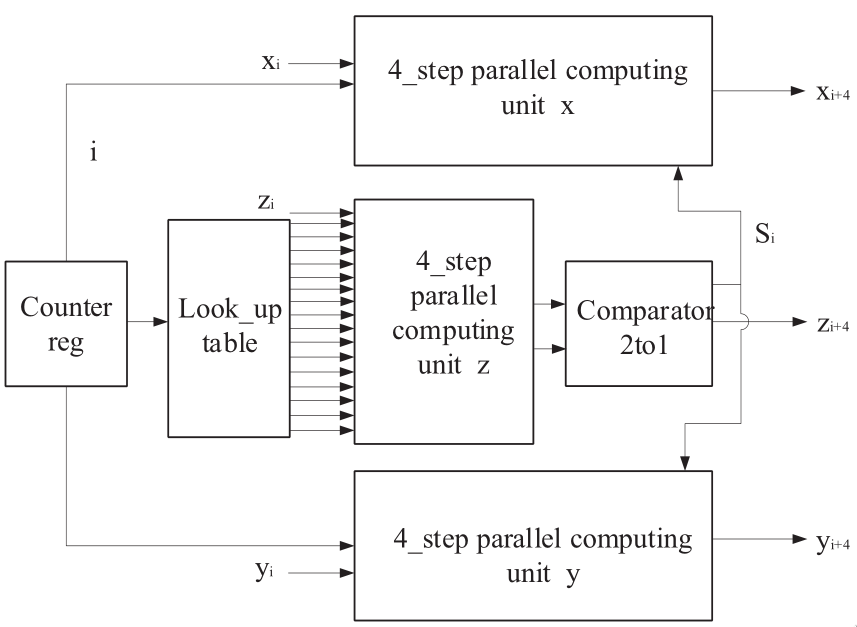
\includegraphics[width=0.75\textwidth]{archivos/CORDIC/2019_4-step-64bit.png}
	\caption{Unidad de procesamiento de \gls{cordic} de doble precisión. Figura extraída de \cite{yeshwanth_high-speed_2018}}
	\label{graf:2019_4-step-64bit}
\end{figure}

\begin{table}[]
	\centering
	\resizebox{\textwidth}{!}{%
		\begin{tabular}{|l|l|l|l|l|l|}
			\hline
			Tipo de \gls{cordic}        & Tradicional & Para-\gls{cordic} & Hybrid & SF \gls{cordic} & Artículo mencionado \\
\hline
			Número de iteraciones & 64          & 17          & 24     & 24        & 15                 
\\ \hline
		\end{tabular}%
	}
	\caption{Número de iteraciones comparando el multiplicador \gls{cordic} con punto flotante de \cite{yeshwanth_high-speed_2018} a otras soluciones.}
	\label{table:2019_4-step-comp-64bit}
\end{table}

Como se comentó anteriormente, \gls{cordic} puede realizar una multitud de operaciones matemáticas según la necesidad del problema. \cite{yeshwanth_high-speed_2018} aprovechan el algoritmo de \gls{cordic} con \textit{pipelining} para optimizar el rendimiento del multiplicador de las mantisas para el \gls{ieee} 754 de 32 bits. Los resultados obtenidos han sido comparados al método de Vedic. Los tiempos de \gls{cordic} son considerablemente mejores, pero ocupa un área en hardware mayor que Vedic.

\begin{table}[]
	\centering
	\resizebox{\textwidth}{!}{%
		\begin{tabular}{|l|l|l|l|}
			\hline
			\multirow{2}{*}{\textbf{Multiplicador punto flotante}} & \multicolumn{3}{l|}{\textbf{Parámetros digitales}}                                  \\ \cline{2-4} 
			& \textbf{Latencia (ns)} & \begin{tabular}[c]{@{}l@{}}Área\\ (\textbf{LUTs})\end{tabular} & \textbf{Consumo (mW)} \\ \hline
			Multiplicador \gls{cordic}                          & 5.259  & 679                                                   & 96    \\ \hline
			Multiplicador Vedic                           & 26.634 & 489                                                   & 95    \\ \hline
		\end{tabular}%
	}
	\label{graf:2018-Vedic-vs-CORDIC}
	\caption{Comparativa entre un multiplicador Vedic y \gls{cordic} de \cite{yeshwanth_high-speed_2018}.}
\end{table}

En el área de la robótica, \cite{evangelista_fully-pipelined_2018} diseñaron en una FPGA una arquitectura basada en CORDIC para la cinemática inversa de un robot hexápodo. El diseño usa numeración de punto flotante de 32 bits, además de \textit{pipelining} para obtener mejoras de frecuencia y \textit{throughput}. Los resultados son comparados a otros robots hexápodo de diferente gama, pero que generalmente tienen procesadores mucho mas potentes y con un gasto energético mucho mas alto. Los resultados además muestran un beneficio en la escalabilidad.

Dentro del trabajo de los radares de apertura sintética (\gls{sar}), \cite{fang_generation_2019} proponen una mejora de los tiempos de cálculo de operaciones trigonométricas, raíces, multiplicación.

El artículo sigue las pautas de muchos otros en diseñar un módulo de pre-procesamiento y post-procesamiento para la conversión de punto flotante a punto fijo y viceversa, con ciertos ajustes para no perder mucha precisión. El diseño fue implementado en una \gls{fpga} para mostrar la eficiencia de uso de espacio de hardware y precisión de los resultados.

\cite{wang_gh_2020} presentan una implementación hardware basado en \gls{cordic} generalizado hiperbólico (GH \gls{cordic}) para el cálculo de raíces cuadradas de base $n$ en punto flotante de precisión simple. Se utilizan múltiples \gls{cordic} en diferentes configuraciones. El cálculo de la raíz en base $n$ se realiza totalmente en punto flotante, sin ningún tipo de conversión a punto fijo. Las operaciones realizadas en el diseño son mas complejas a raíz de operar con el estándar del \gls{ieee}. Además, se usa \textit{pipelining} para mejorar la latencia. El cálculo final son 58 ciclos para una palabra de 32 bits. Los resultados finales del artículo muestran una mejora de \textit{throughput}, eficiencia energética y mejor precisión de los resultados. 














